\documentclass[svgnames,final]{beamer}
\usepackage{etex}
\mode<presentation> {
  \usetheme{I6dv}
}
\usepackage[utf8]{inputenc}
%\usepackage[T1]{fontenc}
\usepackage[english]{babel}
\usepackage{amsmath,amsfonts,amsthm}
\usepackage{mathtools}
\usepackage{booktabs}
\usepackage[orientation=landscape,size=a0,scale=1.4]{beamerposter}
\usepackage{pgfplots}
\usepackage{comment}
% \usepackage{algorithm}
\usepackage[noend]{algpseudocode}
\usepackage{etoolbox}
\pgfplotsset{compat=1.12}
\usepackage{tikz}
\usetikzlibrary{positioning,plotmarks,calc,arrows,decorations.markings,intersections,backgrounds}
\usepackage{amsmath,amsfonts,amsthm,bm} % Math packages
\usepackage{hyperref}
\hypersetup{
    colorlinks=true,
    linkcolor=blue,
    filecolor=magenta,
    urlcolor=cyan,
}

\newcommand{\thetatilde}{\ensuremath{\tilde{\theta}}}
%\tikzexternalize[prefix=tikz_output/]

\usepackage [english]{babel}
\usepackage [autostyle, english = american]{csquotes}
\MakeOuterQuote{"}

\newtoggle{plotexperiments}
\toggletrue{plotexperiments}
%\togglefalse{plotexperiments}

\newcommand{\numplotsamples}{200}

\newcommand{\red}[1]{\textcolor{red}{#1}}
\newcommand{\green}[1]{\textcolor{Green}{#1}}
\newcommand{\blue}[1]{\textcolor{blue}{#1}}
\newcommand{\eps}{\ensuremath{\epsilon}}
\newcommand{\R}{\ensuremath{\mathbb{R}}}
\newcommand{\setC}{\ensuremath{\mathcal{C}}}
\newcommand{\thetahat}{\ensuremath{\hat{\theta}}}
\newcommand{\thetastar}{\ensuremath{\theta^*}}
\newcommand{\Otilde}{\ensuremath{\widetilde{O}}}
\newcommand{\OPT}{\ensuremath{\textnormal{OPT}}}
\newcommand{\projH}{\ensuremath{\mathcal{H}}}
\newcommand{\projT}{\ensuremath{\mathcal{T}}}
\newcommand{\Usubspaces}{\ensuremath{\mathbb{U}}}
\DeclarePairedDelimiter{\abs}{\lvert}{\rvert}
\DeclareMathOperator*{\argmin}{arg\,min}
\DeclarePairedDelimiter{\norm}{\lVert}{\rVert}
\newcommand{\specialcell}[2][c]{%
  \begin{tabular}[#1]{@{}c@{}}#2\end{tabular}}

\newcommand{\prospoint}[1]{\textcolor{Green}{Pros: #1}}
\newcommand{\conspoint}[1]{\textcolor{red}{Cons: #1}}

\newcommand{\greencell}[1]{\green{#1}}
\newcommand{\redcell}[1]{\red{#1}}
\newcommand{\yellowcell}[1]{\textcolor{orange!40!yellow}{#1}}

\title{Graph-Sparse Logistic Regression}
\author{Alexander LeNail$^1$, Ludwig Schmidt$^2$, Jonathan Li$^1$, Tobias Ehrenberger$^1$, Karen Sachs$^1$, Stefanie Jegelka$^2$, Ernest Fraenkel$^1$}
\institute{$^1$MIT BE, $^2$MIT CSAIL}

\begin{document}

\newlength{\gextlength}
\setlength{\gextlength}{14pt}
\newlength{\gselradius}
\setlength{\gselradius}{38pt}

\begin{frame}
\vspace{-.5cm}
\begin{columns}[T]

\begin{column}{.3\linewidth}

	%%%%%%%%%%%%%%%%%%%%%%%%%%%%%%%%%%%%%%%%%%%%%%%%%%%%%%%%%%%%%%%%%%%%%%%%%%%
	\begin{block}{Problem Setup}

    \vspace{-.8cm}

    \textbf{Variable selection} in a linear model:
    {\Large
    \[
      y \; = \; \sigma(X \,  \thetastar)
    \]
    }

    \vspace{-.7cm}

    \begin{itemize}
      \item Data matrix $X \in \R^{n \times d}$\\[.2cm]
      \item Unknown parameters $\thetastar \in \R^d$\\[.2cm]
      \item Binary labels $y \in \{0,1\}^n$\\[.2cm]
      \item $\sigma: \R \rightarrow \R$ is the logistic function $\sigma(x) = \frac{1}{1 + e^{-x}}$
    \end{itemize}

    \vspace{1.2cm}
    \textbf{This work:} our goal is to select a \textbf{graph-sparse} set of variables.\\[.5cm]
    $\quad\rightarrow$ \textbf{Statistical efficiency:} fewer variables for same error.\\[.3cm]
    $\quad\rightarrow$ \textbf{Interpretability:} graph-structure in many applications.

    \vspace{1.2cm}
    \textbf{Graph sparsity}
		\begin{itemize}
  		\item Every variable (parameter index) corresponds to a node.\\[.2cm]
			\item Selected variables form a \textbf{connected subgraph.}
    \end{itemize}

    \begin{columns}
\column{.5\textwidth}
  \begin{center}
  \begin{tikzpicture}[scale=1.5]
  \tikzstyle{mythick}=[line width=.12cm];
  \tikzstyle{gn}=[draw=black,circle,inner sep=1pt,minimum size=.9cm,mythick]
  \tikzstyle{ed}=[draw=black,mythick]
  \tikzstyle{selection}=[double=blue!20,double distance=34pt,mythick,draw=blue!50,line cap=round,line join=round];
  \node [gn] (a) at (0,0) {};
  \node [gn] (b) at (3,0) {};
  \node [gn] (c) at (2,2.8) {};
  \node [gn] (d) at (3.5,1.7) {};
  \node [gn] (e) at (-1.4, 1) {};
  \node [gn] (f) at (.4,3.0) {};
  \node [gn] (g) at (.3,1.8) {};
  \node [gn] (h) at (-.6,2.3) {};
  \draw [ed] (a) -- (b);
  \draw [ed] (c) -- (d);
  \draw [ed] (a) -- (e);
  \draw [ed] (d) -- (b);
  \draw [ed] (a) -- (c);
  \draw [ed] (b) -- (c);
  \draw [ed] (a) -- (g);
  \draw [ed] (g) -- (c);
  \draw [ed] (g) -- (h);
  \draw [ed] (e) -- (h);
  \draw [ed] (f) -- (h);
  \begin{scope}[on background layer]
  \draw [selection] (-.6,2.3) -- (-1.4,1) -- (0,0);
  \end{scope}
  \end{tikzpicture}

  \green{Graph-sparse}\\[.5cm]
  \end{center}
\column{.5\textwidth}
  \begin{center}
  \begin{tikzpicture}[scale=1.5]
  \tikzstyle{mythick}=[line width=.12cm];
  \tikzstyle{gn}=[draw=black,circle,mythick,inner sep=1pt,minimum size=.9cm]
  \tikzstyle{ed}=[draw=black,mythick]
  \tikzstyle{selection}=[double=blue!20,double distance=9pt,mythick,draw=blue!50,line cap=round,line join=round];
  \node [gn] (a) at (0,0) {};
  \node [gn] (b) at (3,0) {};
  \node [gn] (c) at (2,2.8) {};
  \node [gn] (d) at (3.5,1.7) {};
  \node [gn] (e) at (-1.4, 1) {};
  \node [gn] (f) at (.4,3.0) {};
  \node [gn] (g) at (.3,1.8) {};
  \node [gn] (h) at (-.6,2.3) {};
  \draw [ed] (a) -- (b);
  \draw [ed] (c) -- (d);
  \draw [ed] (a) -- (e);
  \draw [ed] (d) -- (b);
  \draw [ed] (a) -- (c);
  \draw [ed] (b) -- (c);
  \draw [ed] (a) -- (g);
  \draw [ed] (g) -- (c);
  \draw [ed] (g) -- (h);
  \draw [ed] (e) -- (h);
  \draw [ed] (f) -- (h);
  \begin{scope}[on background layer]
  \node [circle,mythick,draw=blue!50,fill=blue!20,inner sep=0pt,minimum size=\gselradius] at (f) {};
  \node [circle,mythick,draw=blue!50,fill=blue!20,inner sep=0pt,minimum size=\gselradius] at (b) {};
  \node [circle,mythick,draw=blue!50,fill=blue!20,inner sep=0pt,minimum size=\gselradius] at (g) {};
  \end{scope}
  \end{tikzpicture}

  \red{Not graph-sparse}
  \end{center}
\end{columns}


	\end{block}

	\vspace{1.0cm}

	%%%%%%%%%%%%%%%%%%%%%%%%%%%%%%%%%%%%%%%%%%%%%%%%%%%%%%%%%%%%%%%%%%%%%%%%%%%
	\begin{block}{Motivation: graph-structed data in biology}
		Protein expression data with a \textbf{protein-protein interation network.}\\[-.2cm]
		\begin{figure}[h]
		\centering
		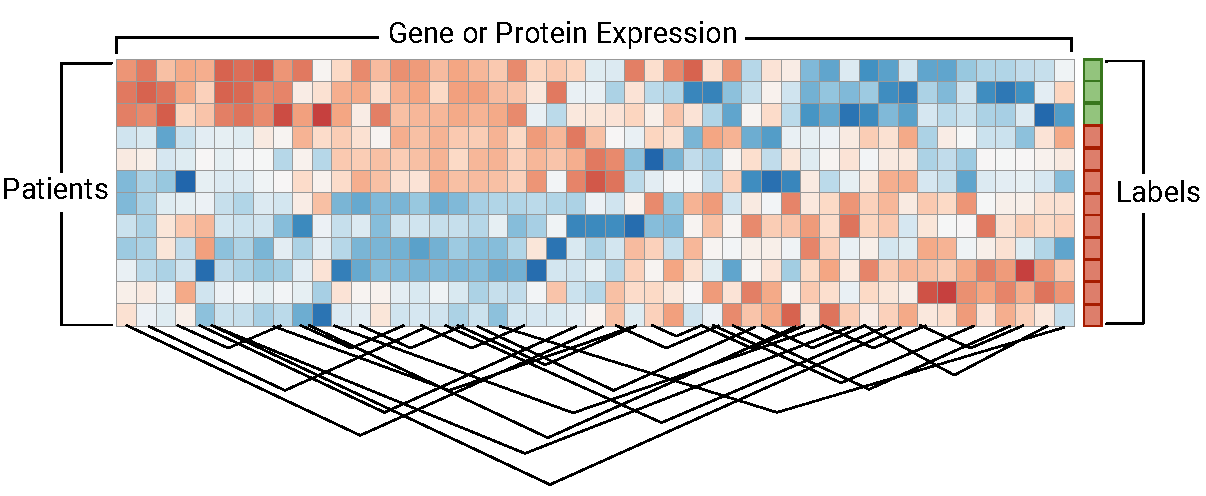
\includegraphics[width=.8\linewidth]{images/matrix.pdf}
		\end{figure}

		Graph given by prior knowledge from biology:\\[-.6cm]

		\begin{figure}[h]
		\centering
		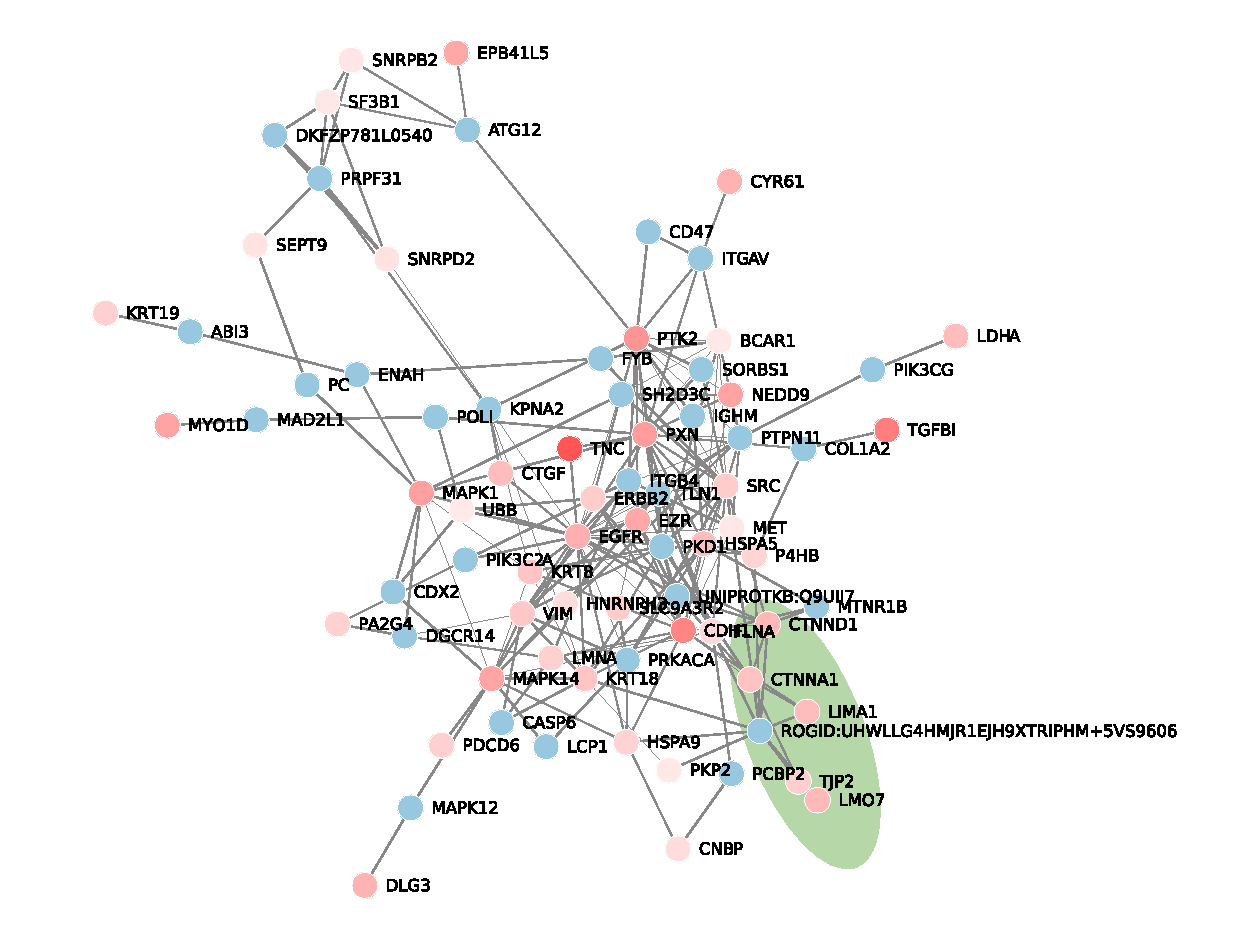
\includegraphics[width=0.7\linewidth]{images/graph.pdf}
		\end{figure}

		\vspace{-1.5cm}

	\end{block}

	\vspace{2cm}

\end{column}

\begin{column}{.3\linewidth}

	%%%%%%%%%%%%%%%%%%%%%%%%%%%%%%%%%%%%%%%%%%%%%%%%%%%%%%%%%%%%%%%%%%%%%%%%%%%
	\begin{block}{Approach}
    We build on results in \textbf{compressive sensing} for graph-sparse data.\\[.3cm]
		$\qquad$\textcolor{darkgray}{[Huang, Zhang, Metaxas, 2011], [Hegde, Indyk, Schmidt, 2015]}
		\vspace{1.2cm}

		$\rightarrow$ We introduce \textbf{Graph-Sparse Logistic Regression} (GSLR).\\[.2cm]
		\begin{itemize}
			\item Gradient descent on logistic loss.\\[.2cm]
			\item Efficient projections onto the graph sparse set.
		\end{itemize}

		\vspace{1cm}

		\begin{tikzpicture}
    \node [rectangle,draw,black,line width=.2cm,text width=33cm,align=left] {\begin{algorithmic}[1]
			\vspace{-.3cm}
			\Function{GSLR}{$X$, $y$, $G$, $s$, $\eta$, $k$}
			\State Let $f(X, y, \theta)$ be the logistic loss.
			\State $\thetahat^0 \gets 0$
			\For{$i \gets 0, \ldots, k-1$}
			\State $\thetatilde^{i+1} \gets \thetahat^i - \eta \cdot \nabla f(X, y, \thetahat^i)$
			\State $\thetahat^{i+1} \gets P_{G,s}(\thetatilde^{i+1})$ \Comment{Graph-sparse projection \hspace{.5cm}$ \;$ }
			\EndFor
			\State \textbf{return} $\thetahat^k$
			\EndFunction
			\vspace{.7cm}
			\end{algorithmic}};
    \end{tikzpicture}
	\end{block}

	\vspace{1.0cm}

	%%%%%%%%%%%%%%%%%%%%%%%%%%%%%%%%%%%%%%%%%%%%%%%%%%%%%%%%%%%%%%%%%%%%%%%%%%%
	\begin{block}{Efficient Graph-Sparse Projections}
	\vspace{-.5cm}
	\textbf{Projection problem}: Given $b \in \R^d$ and a graph-sparse set $\mathbb{G}$, find
	{\Large
	\[
		\Omega^* \; = \; \argmin_{\Omega \in \mathbb{G}} \, \norm{b  - b_{\Omega}} \; .
	\]
	}
	
\begin{columns}
\begin{column}{.5\linewidth}
\begin{center}
\begin{tikzpicture}[scale=2.5]
\tikzstyle{mythick}=[line width=.12cm];
\tikzstyle{gn}=[draw=black,circle,thick,inner sep=7pt,minimum size=1cm,mythick]
\tikzstyle{ed}=[draw=black,mythick]
\node [gn] (a) at (0,0) {$3$};
\node [gn] (b) at (3,0) {$5$};
\node [gn] (c) at (2,2.8) {$7$};
\node [gn] (d) at (3.5,1.7) {$2$};
\node [gn] (e) at (-1.4, 1) {$6$};
\node [gn] (f) at (.4,3.0) {$8$};
\node [gn] (g) at (.3,1.8) {$1$};
\node [gn] (h) at (-.6,2.3) {$0$};
\draw [ed] (a) -- (b);
\draw [ed] (c) -- (d);
\draw [ed] (a) -- (e);
\draw [ed] (d) -- (b);
\draw [ed] (a) -- (c);
\draw [ed] (b) -- (c);
\draw [ed] (a) -- (g);
\draw [ed] (g) -- (c);
\draw [ed] (g) -- (h);
\draw [ed] (e) -- (h);
\draw [ed] (f) -- (h);
\end{tikzpicture}

Input
\end{center}
\end{column}
\begin{column}{.5\linewidth}
\begin{center}
\begin{tikzpicture}[scale=2.5]
\tikzstyle{mythick}=[line width=.12cm];
\tikzstyle{gn}=[draw=black,circle,thick,inner sep=7pt,minimum size=1cm,mythick]
\tikzstyle{ed}=[draw=black,mythick]
\tikzstyle{selection}=[double=blue!20,double distance=60pt,line width=.2cm,draw=blue!50,line cap=round,line join=round];
\node [gn] (a) at (0,0) {$3$};
\node [gn] (b) at (3,0) {$5$};
\node [gn] (c) at (2,2.8) {$7$};
\node [gn] (d) at (3.5,1.7) {$2$};
\node [gn] (e) at (-1.4, 1) {$6$};
\node [gn] (f) at (.4,3.0) {$8$};
\node [gn] (g) at (.3,1.8) {$1$};
\node [gn] (h) at (-.6,2.3) {$0$};
\draw [ed] (a) -- (b);
\draw [ed] (c) -- (d);
\draw [ed] (a) -- (e);
\draw [ed] (d) -- (b);
\draw [ed] (a) -- (c);
\draw [ed] (b) -- (c);
\draw [ed] (a) -- (g);
\draw [ed] (g) -- (c);
\draw [ed] (g) -- (h);
\draw [ed] (e) -- (h);
\draw [ed] (f) -- (h);
\begin{scope}[on background layer]
\draw [selection] (0,0) -- (3,0) -- (2,2.8);
\end{scope}
\end{tikzpicture}

Output
\end{center}
\end{column}
\end{columns}

\vspace{1.2cm}

We solve \textbf{approximate} versions of the projection problem via reductions to the \textbf{prize-collecting Steiner tree problem} (PCST).\\[1.5cm]

\textbf{Objective of PCST:} Given a graph with edge costs $c$ and node prizes $\pi$, find a subtree $T$ minimizing $c(T) + \pi(\overline{T})$.

\vspace{.7cm}

\begin{columns}
\begin{column}{.5\linewidth}
\begin{center}
\begin{tikzpicture}[scale=2.5]
\tikzstyle{mythick}=[line width=.12cm];
\tikzstyle{gn}=[draw=black,circle,thick,inner sep=7pt,minimum size=1cm,mythick,text=red]
\tikzstyle{ed}=[draw=black,mythick]
\tikzstyle{selection}=[double=blue!20,double distance=60pt,line width=.2cm,draw=blue!50,line cap=round,line join=round];
\node [gn] (a) at (0,0) {7};
\node [gn] (b) at (3,0) {6};
\node [gn] (c) at (2,2.8) {2};
\node [gn] (d) at (3.5,1.7) {5};
\node [gn] (e) at (-1.4, 1) {4};
\node [gn] (f) at (.4,3.0) {1};
\node [gn] (g) at (.3,1.8) {8};
\node [gn] (h) at (-.6,2.3) {3};
\draw [ed] (a) -- (b) node [below,midway] {1};
\draw [ed] (c) -- (d) node [above,midway,xshift=10pt,yshift=-4pt] {2};
\draw [ed] (a) -- (e) node [below=-7.5pt,midway,xshift=-10pt] {3};
\draw [ed] (d) -- (b) node [below=-20pt,midway,xshift=14pt] {4};
\draw [ed] (a) -- (c) node [below=-4pt,midway,xshift=10pt] {5};
\draw [ed] (b) -- (c) node [above=-4pt,midway,xshift=9pt] {6};
\draw [ed] (a) -- (g) node [above=-10pt,midway,xshift=-14pt] {7};
\draw [ed] (g) -- (c) node [above,midway,xshift=-2pt] {8};
\draw [ed] (g) -- (h) node [above=-4pt,midway,xshift=8pt] {9};
\draw [ed] (e) -- (h) node [above=-10pt,midway,xshift=-20pt] {10};
\draw [ed] (f) -- (h) node [above=-2pt,midway,xshift=-11pt] {11};
\end{tikzpicture}

Input
\end{center}
\end{column}
\begin{column}{.5\linewidth}
\begin{center}
\begin{tikzpicture}[scale=2.5]
\tikzstyle{mythick}=[line width=.12cm];
\tikzstyle{gn}=[draw=black,circle,thick,inner sep=7pt,minimum size=1cm,mythick,text=red]
\tikzstyle{ed}=[draw=black,mythick]
\tikzstyle{selection}=[double=blue!20,double distance=60pt,line width=.2cm,draw=blue!50,line cap=round,line join=round];
\node [gn] (a) at (0,0) {7};
\node [gn] (b) at (3,0) {6};
\node [gn] (c) at (2,2.8) {2};
\node [gn] (d) at (3.5,1.7) {5};
\node [gn] (e) at (-1.4, 1) {4};
\node [gn] (f) at (.4,3.0) {1};
\node [gn] (g) at (.3,1.8) {8};
\node [gn] (h) at (-.6,2.3) {3};
\draw [ed] (a) -- (b) node [below,midway] {1};
\draw [ed] (c) -- (d) node [above,midway,xshift=10pt,yshift=-4pt] {2};
\draw [ed] (a) -- (e) node [below=-7.5pt,midway,xshift=-10pt] {3};
\draw [ed] (d) -- (b) node [below=-20pt,midway,xshift=14pt] {4};
\draw [ed] (a) -- (c) node [below=-4pt,midway,xshift=10pt] {5};
\draw [ed] (b) -- (c) node [above=-4pt,midway,xshift=9pt] {6};
\draw [ed] (a) -- (g) node [above=-10pt,midway,xshift=-14pt] {7};
\draw [ed] (g) -- (c) node [above,midway,xshift=-2pt] {8};
\draw [ed] (g) -- (h) node [above=-4pt,midway,xshift=8pt] {9};
\draw [ed] (e) -- (h) node [above=-10pt,midway,xshift=-20pt] {10};
\draw [ed] (f) -- (h) node [above=-2pt,midway,xshift=-11pt] {11};
\begin{scope}[on background layer]
\draw [selection] (3.5,1.7) -- (3,0) -- (0,0) -- (-1.4,1) -- (0,0) -- (.3,1.8);
\end{scope}
\end{tikzpicture}

Output
\end{center}
\end{column}
\end{columns}

\vspace{1.5cm}

$\rightarrow$ \textbf{Nearly-linear} time approximate projections.

	\end{block}
\end{column}

\begin{column}{.3\linewidth}

	%%%%%%%%%%%%%%%%%%%%%%%%%%%%%%%%%%%%%%%%%%%%%%%%%%%%%%%%%%%%%%%%%%%%%%%%%%%
	\begin{block}{Experimental Setup}

		Since we don't have the ground truth subgraphs for the real Ovarian Cancer data,
		we generate synthetic data by this procedure:

		1. Determine $\mu$ and $\bm{\Sigma}$ from real Ovarian Cancer Proteomics data.

		2. Sample from multivariate $\mathcal{N} (\vec{\mu}, \bm{\Sigma} )$

		3. Sample perturbation vector $\vec{x}$:

			\setlength\parindent{96pt}

			scheme 1: $\vec{x_p} = \mathcal{N} (0, \sigma_p^2 )$ if $p \in$ KEGG, 0 otherwise

			scheme 2: $\vec{x_p} = \mathcal{N} (\pm\sigma_p, \sigma_p^2 )$ if $p \in$ KEGG, 0 otherwise

			\setlength\parindent{0pt}

		4. Translate "positive" samples by perturbation vector


		\begin{figure}[h]
		  \centering
		\begin{tikzpicture}[
		declare function={mu1=1;},
		declare function={mu2=2;},
		declare function={mu3=2;},
		declare function={sigma1=0.5;},
		declare function={sigma2=1;},
		declare function={normal(\m,\s)=1/(2*\s*sqrt(pi))*exp(-(x-\m)^2/(2*\s^2));},
		declare function={bivar(\ma,\sa,\mb,\sb)=3.3/(2*pi*\sa*\sb) * exp(-((x-\ma)^2/\sa^2 + (y-\mb)^2/\sb^2))/2;}]
		\begin{axis}[
		ticks=none,
		colormap name=whitered,
		width=18cm,
		view={35}{65},
		enlargelimits=false,
		grid=major,
		domain=-1:4,
		y domain=-1:4,
		samples=26,
		xlabel=$x_1$,
		ylabel=$x_2$,
		zlabel={$P$},
		]

		\addplot3 [opacity=1,surf,colormap={whitered}{color(0cm)=(white); color(1cm)=(orange!75!red)}] {bivar(mu1,sigma1,mu2,sigma2)};
		\addplot3 [opacity=0.5,surf,colormap={whiteyellow}{color(0cm)=(white); color(1cm)=(orange!75!yellow)}] {bivar(mu3,sigma1,mu2,sigma2)};

		\addplot3 [domain=-1:4,samples=31, samples y=0, thin, smooth] (x,4,{normal(mu1,sigma1)});
		\addplot3 [domain=-1:4,samples=31, samples y=0, thin, smooth] (-1,x,{normal(mu2,sigma2)});
		\addplot3 [domain=-1:4,samples=31, samples y=0, thin, smooth] (x,4,{normal(mu3,sigma1)});

		\draw [black!50] (axis cs:-1,0,0) -- (axis cs:4,0,0);
		\draw [black!50] (axis cs:0,-1,0) -- (axis cs:0,4,0);

		\end{axis}
		\end{tikzpicture}
		\end{figure}


		Since we know the perturbation vector, we know the ground truth!

		We can then evaluate algorithms on the feature selection task.

	\end{block}

	\vspace{1.0cm}

	%%%%%%%%%%%%%%%%%%%%%%%%%%%%%%%%%%%%%%%%%%%%%%%%%%%%%%%%%%%%%%%%%%%%%%%%%%%
	\begin{block}{Experimental Results}

		We benchmark GSLR against the LASSO by how many of the truly "perturbed" features each uses in its support.

		\begin{figure}[h]
		\centering
		%\begin{subfigure}{.5\textwidth}
		%  \centering
		  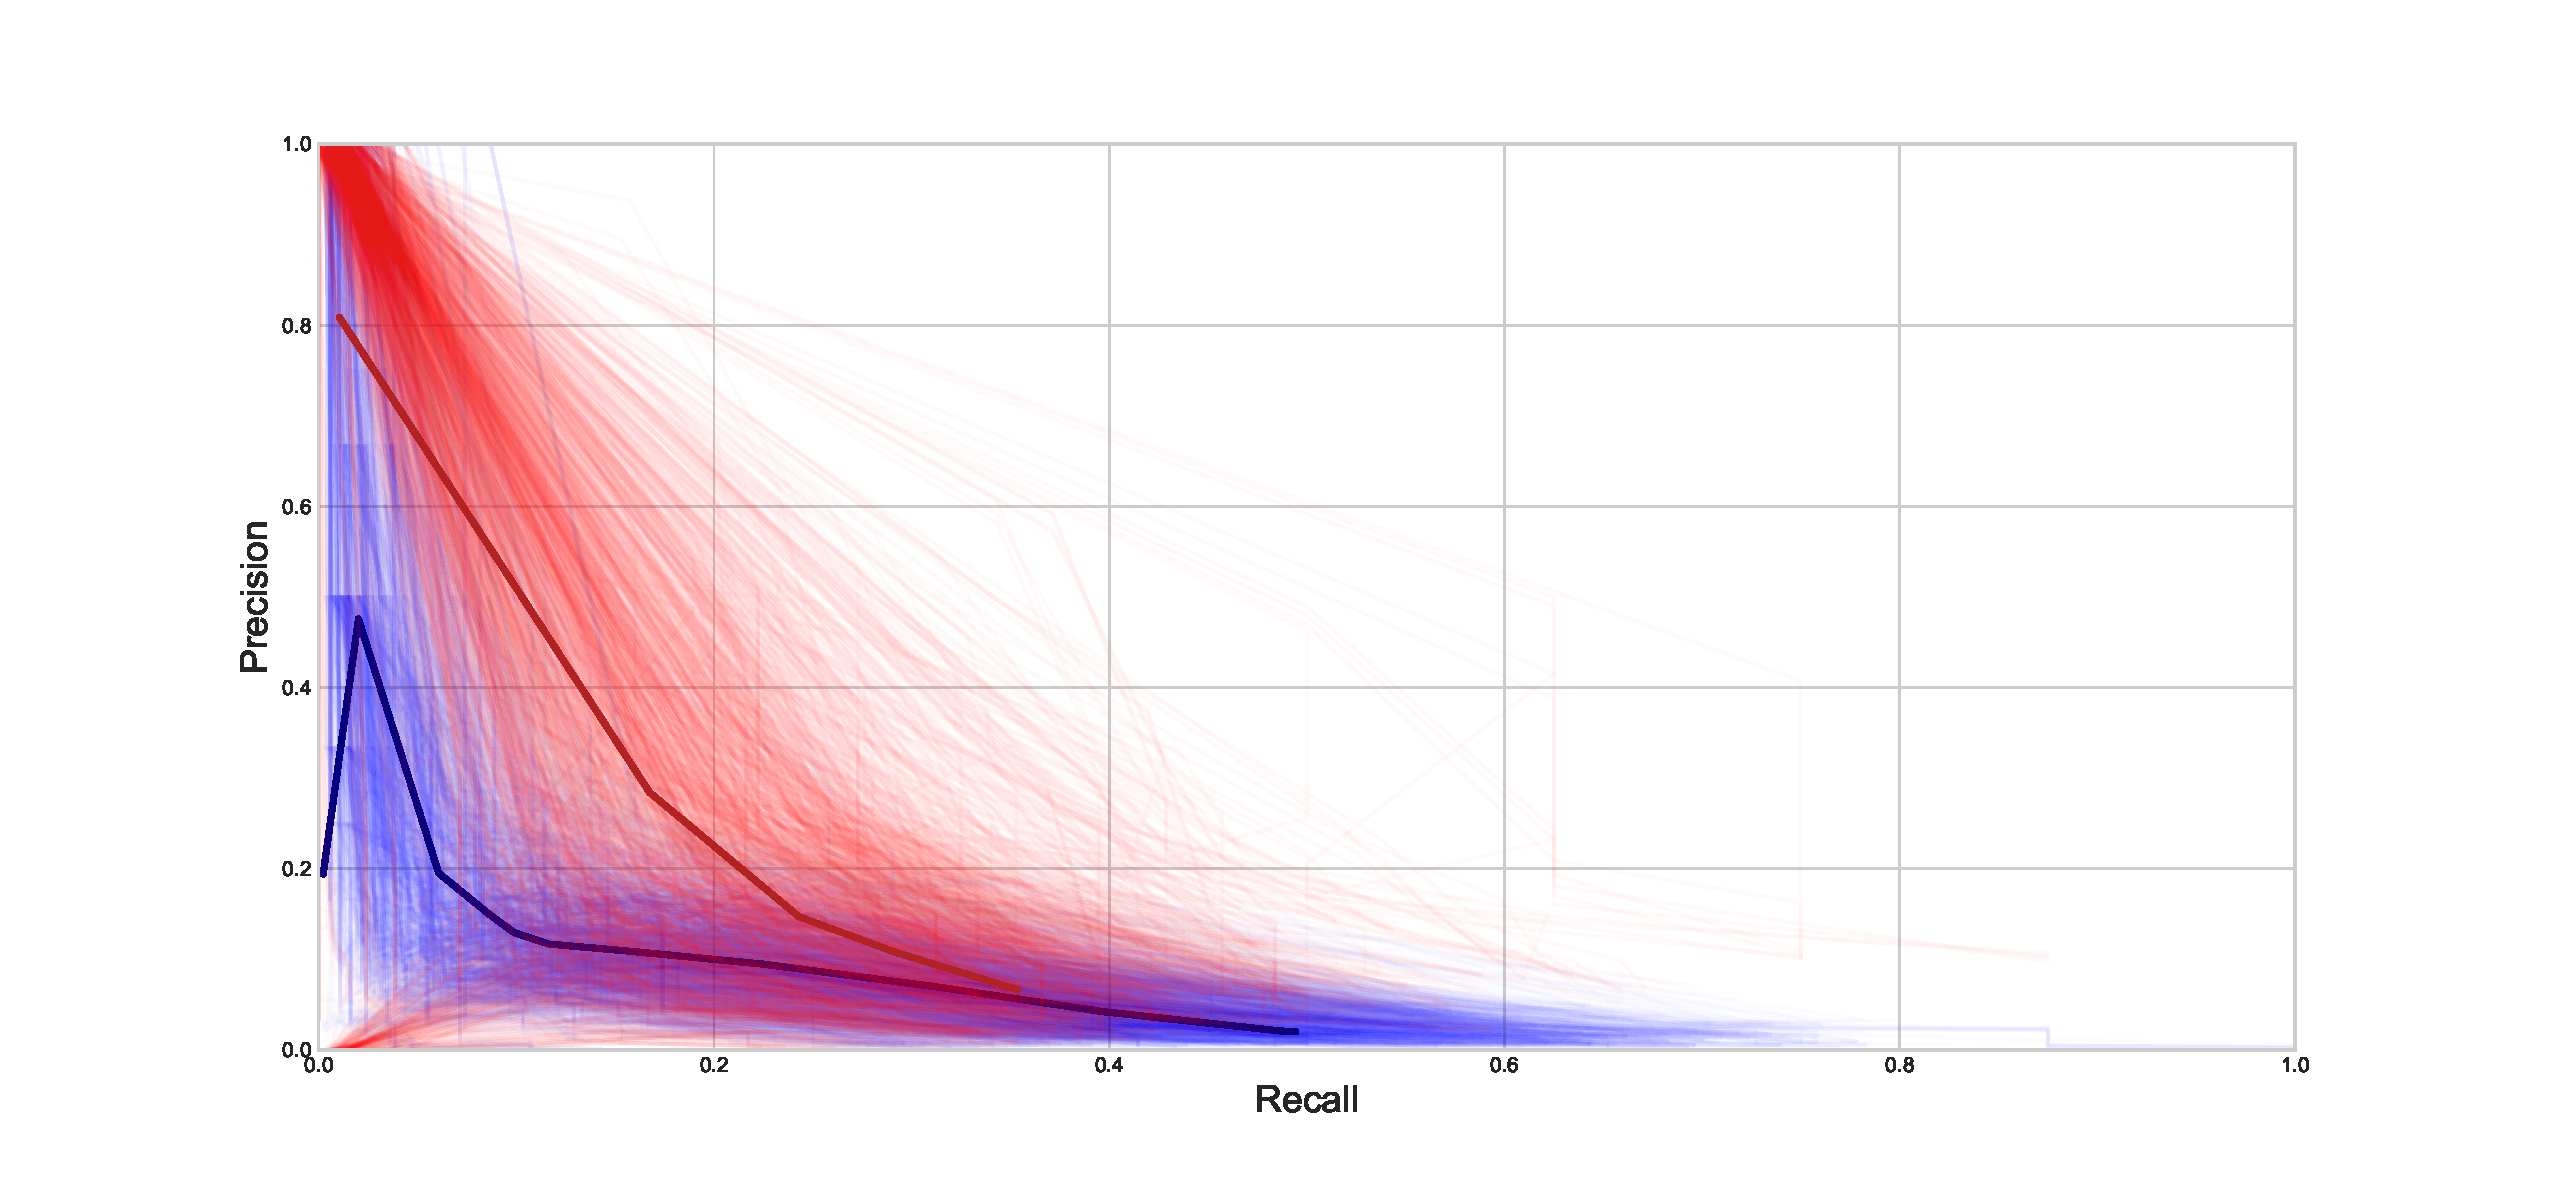
\includegraphics[width=.5\linewidth]{images/2.pdf}
		%\end{subfigure}%
		%\begin{subfigure}{.5\textwidth}
		%  \centering
		  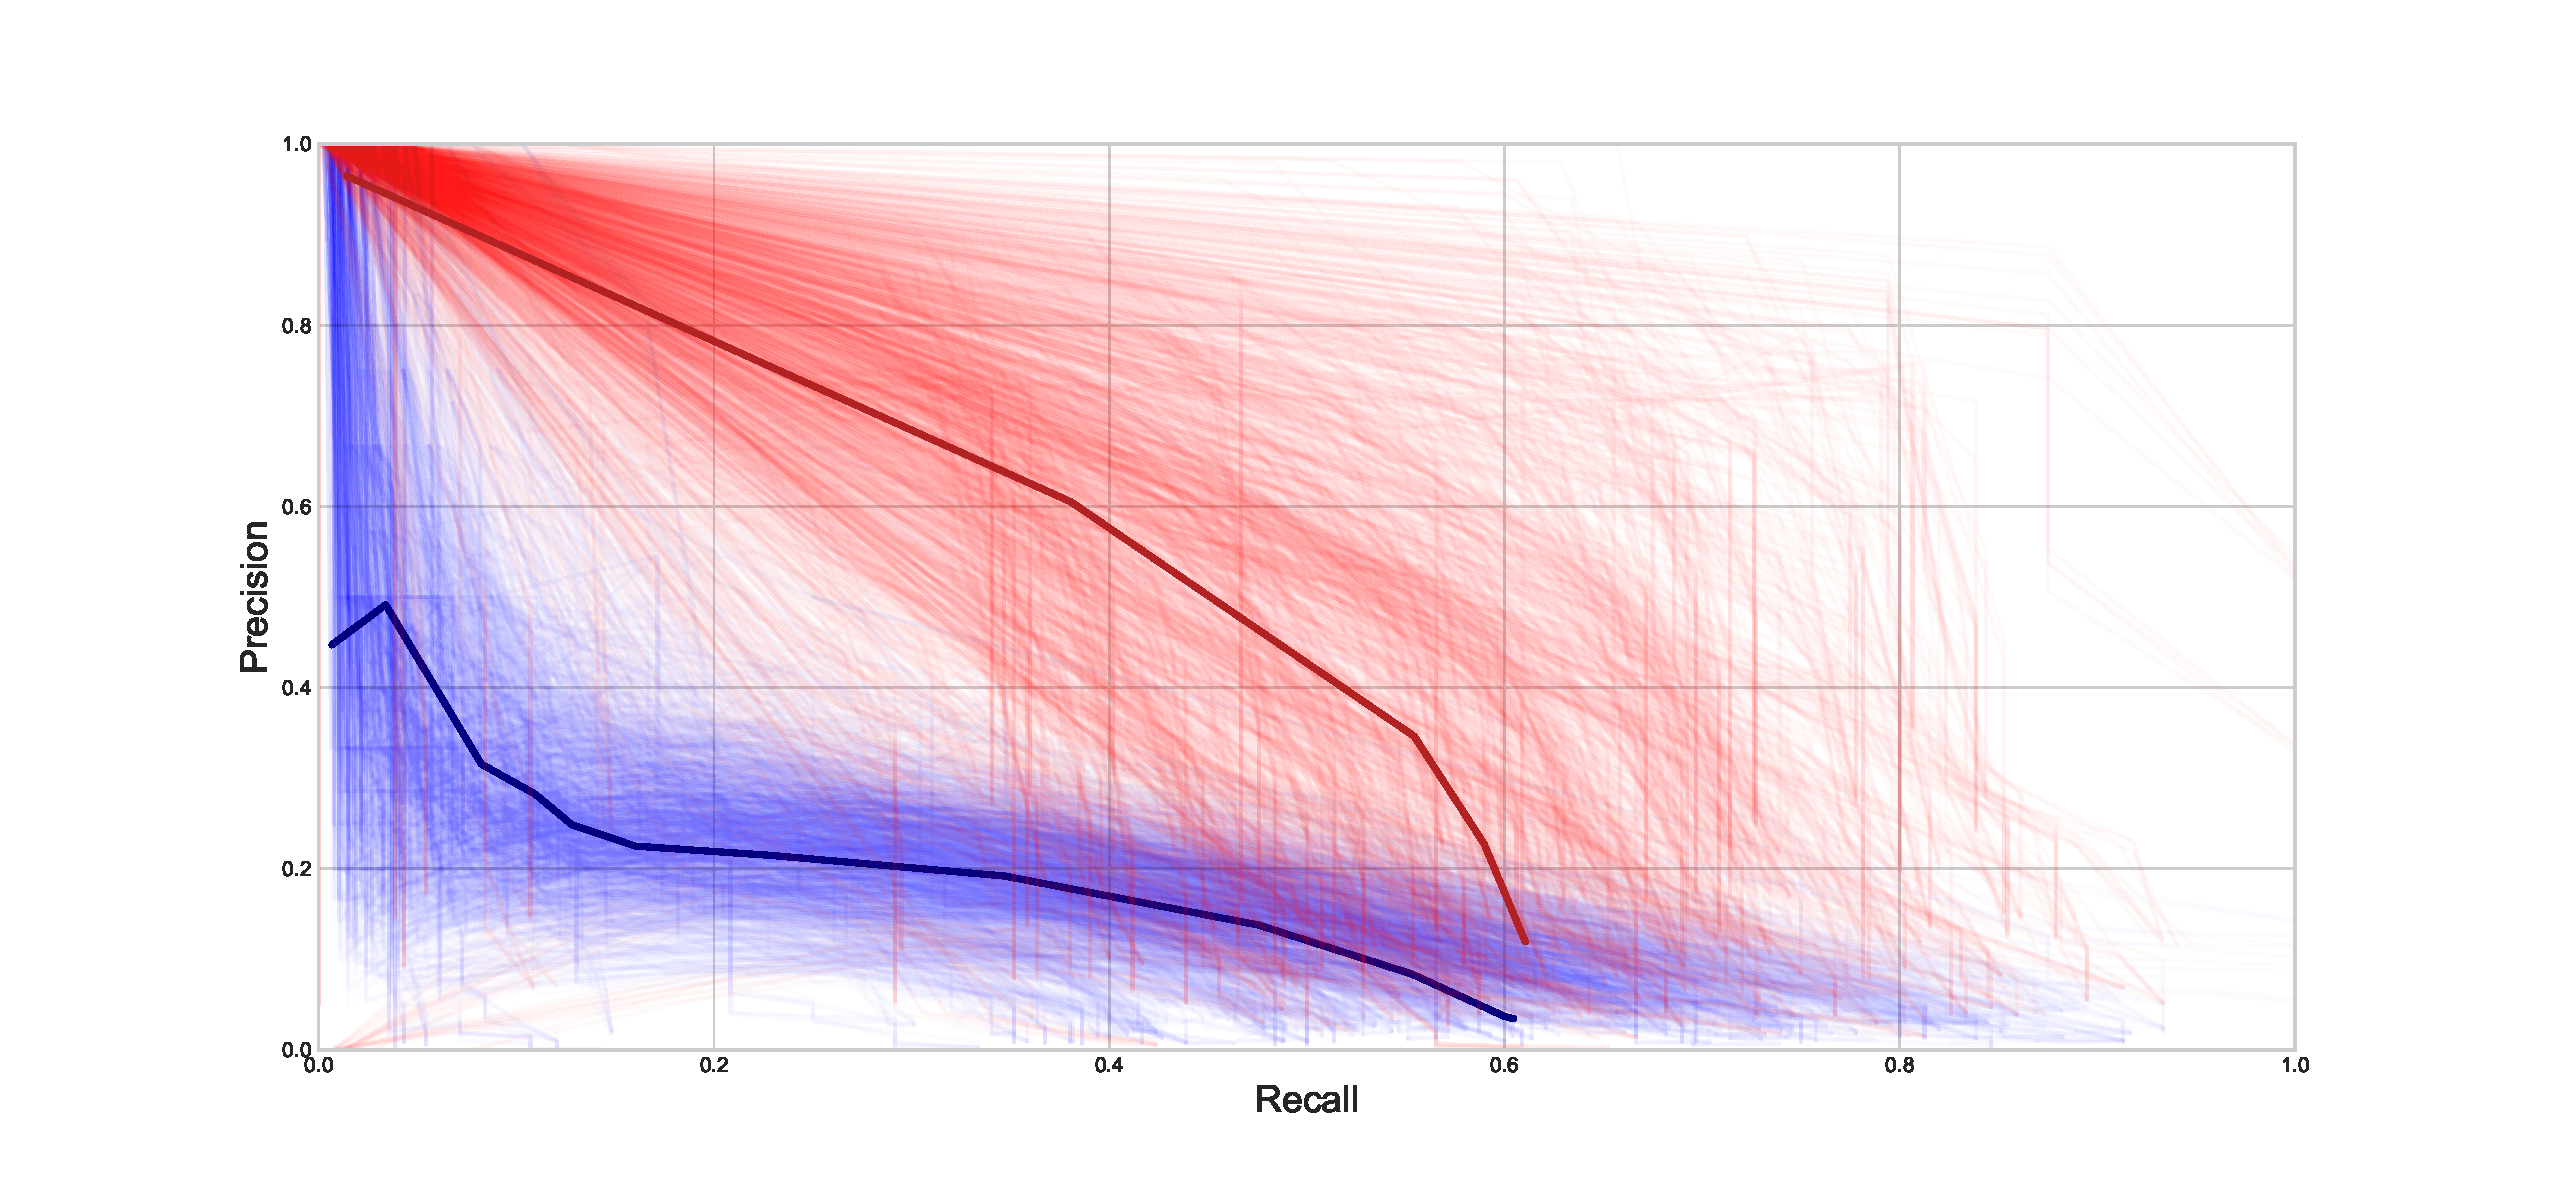
\includegraphics[width=.5\linewidth]{images/1.pdf}
    \newline
		%\end{subfigure}
		%\begin{subfigure}{.5\textwidth}
		%  \centering
		  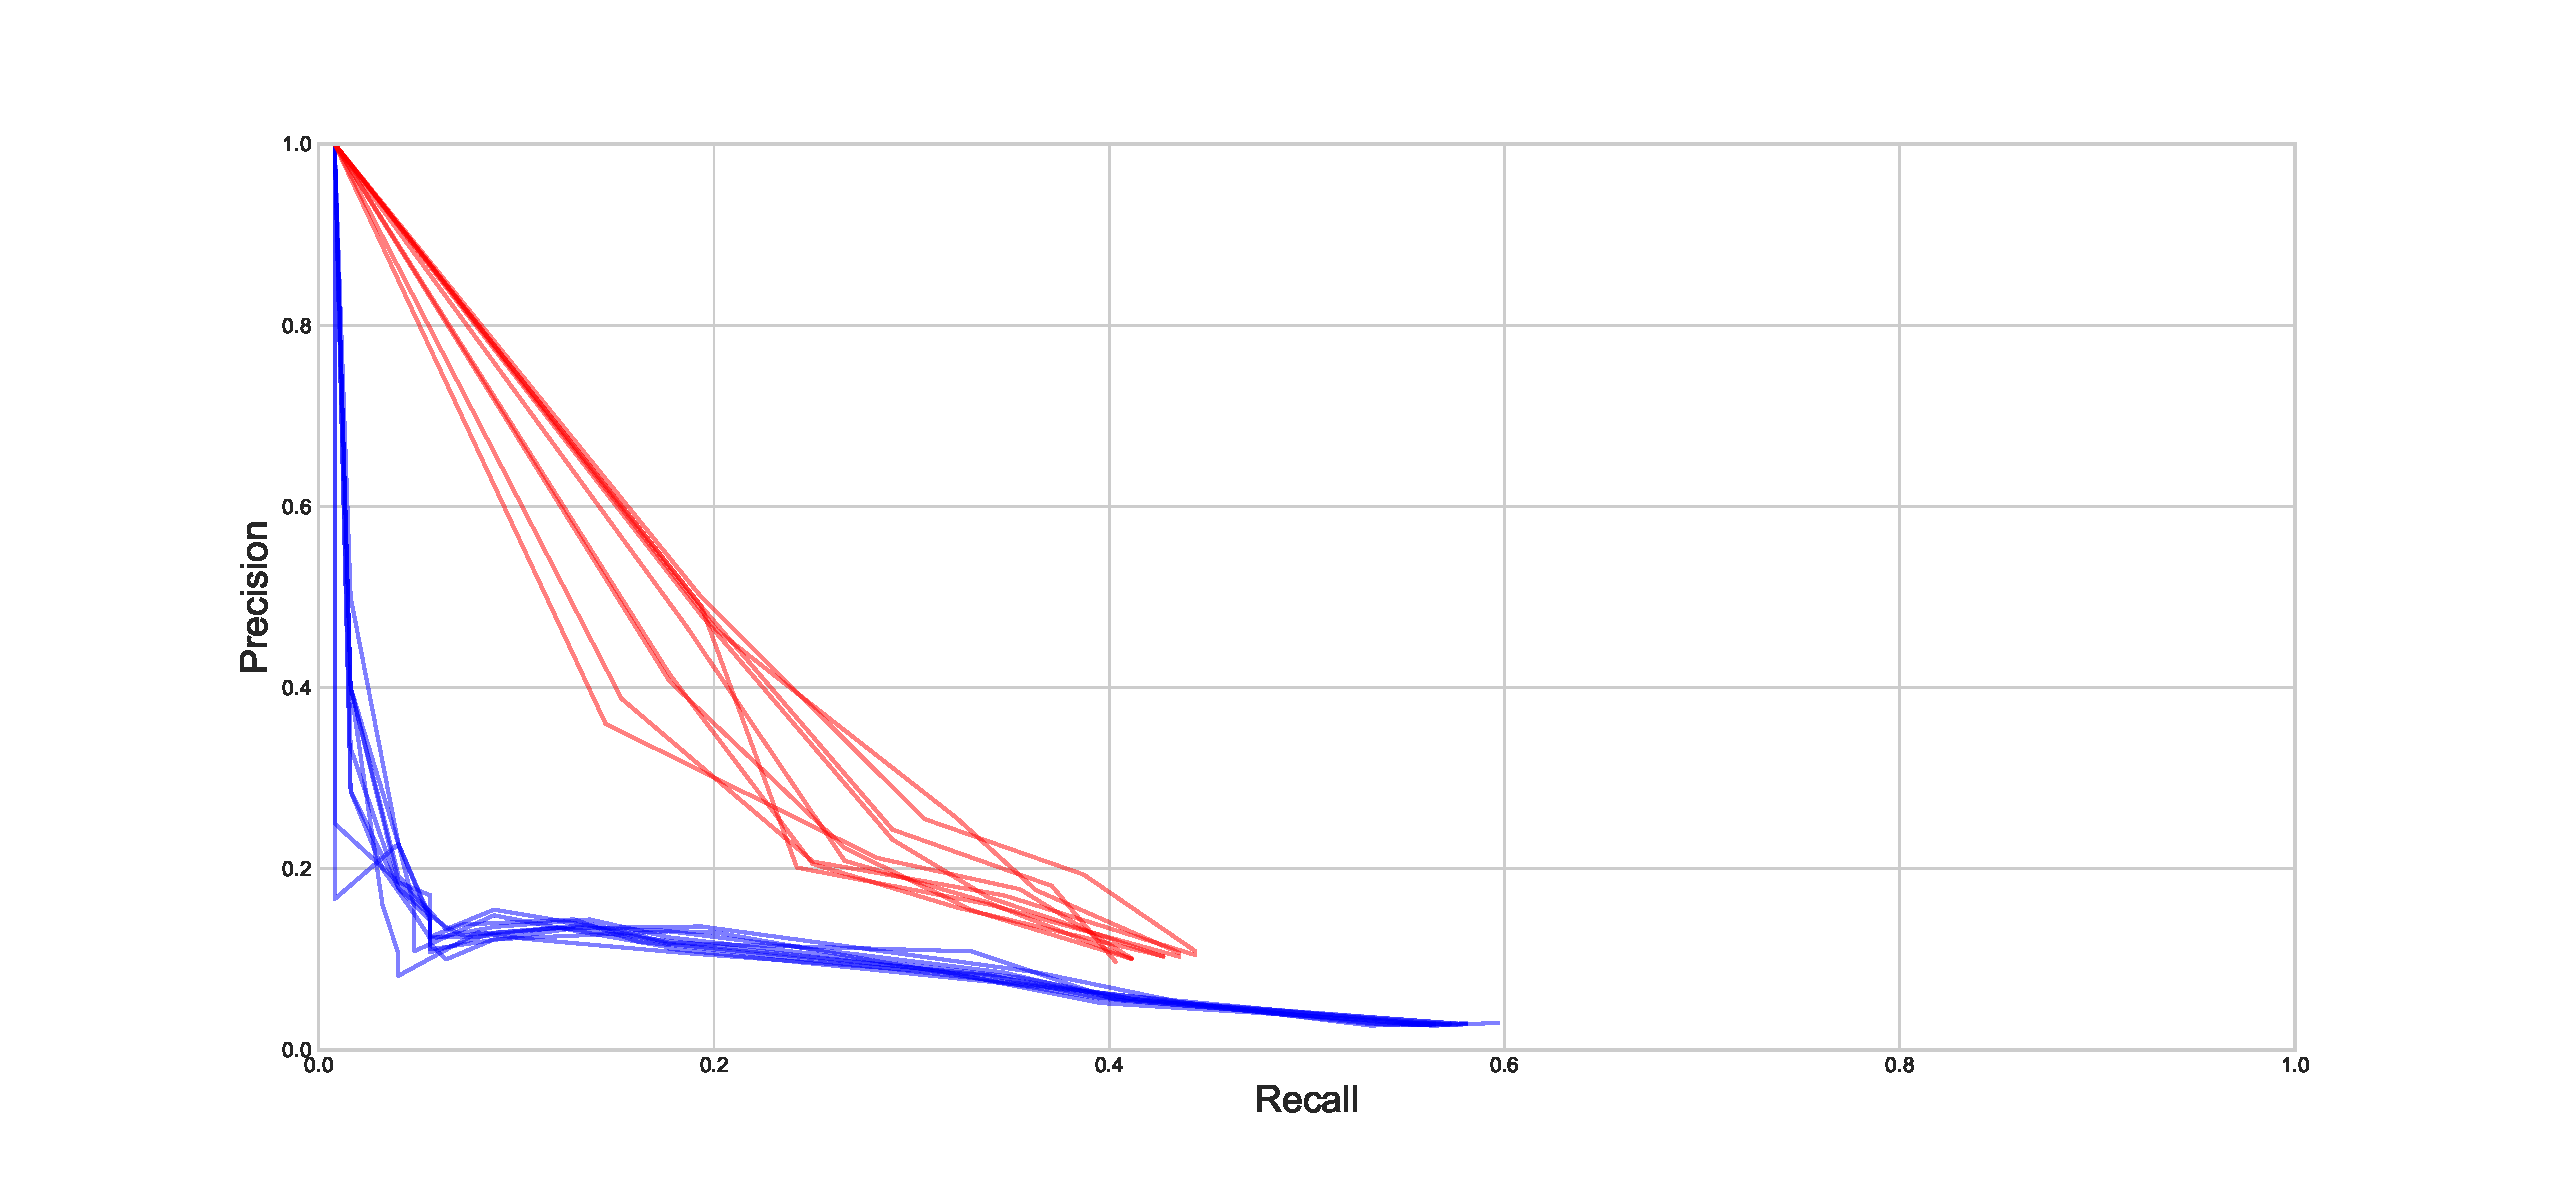
\includegraphics[width=.5\linewidth]{images/4.pdf}
		%\end{subfigure}%
		%\begin{subfigure}{.5\textwidth}
		%  \centering
		  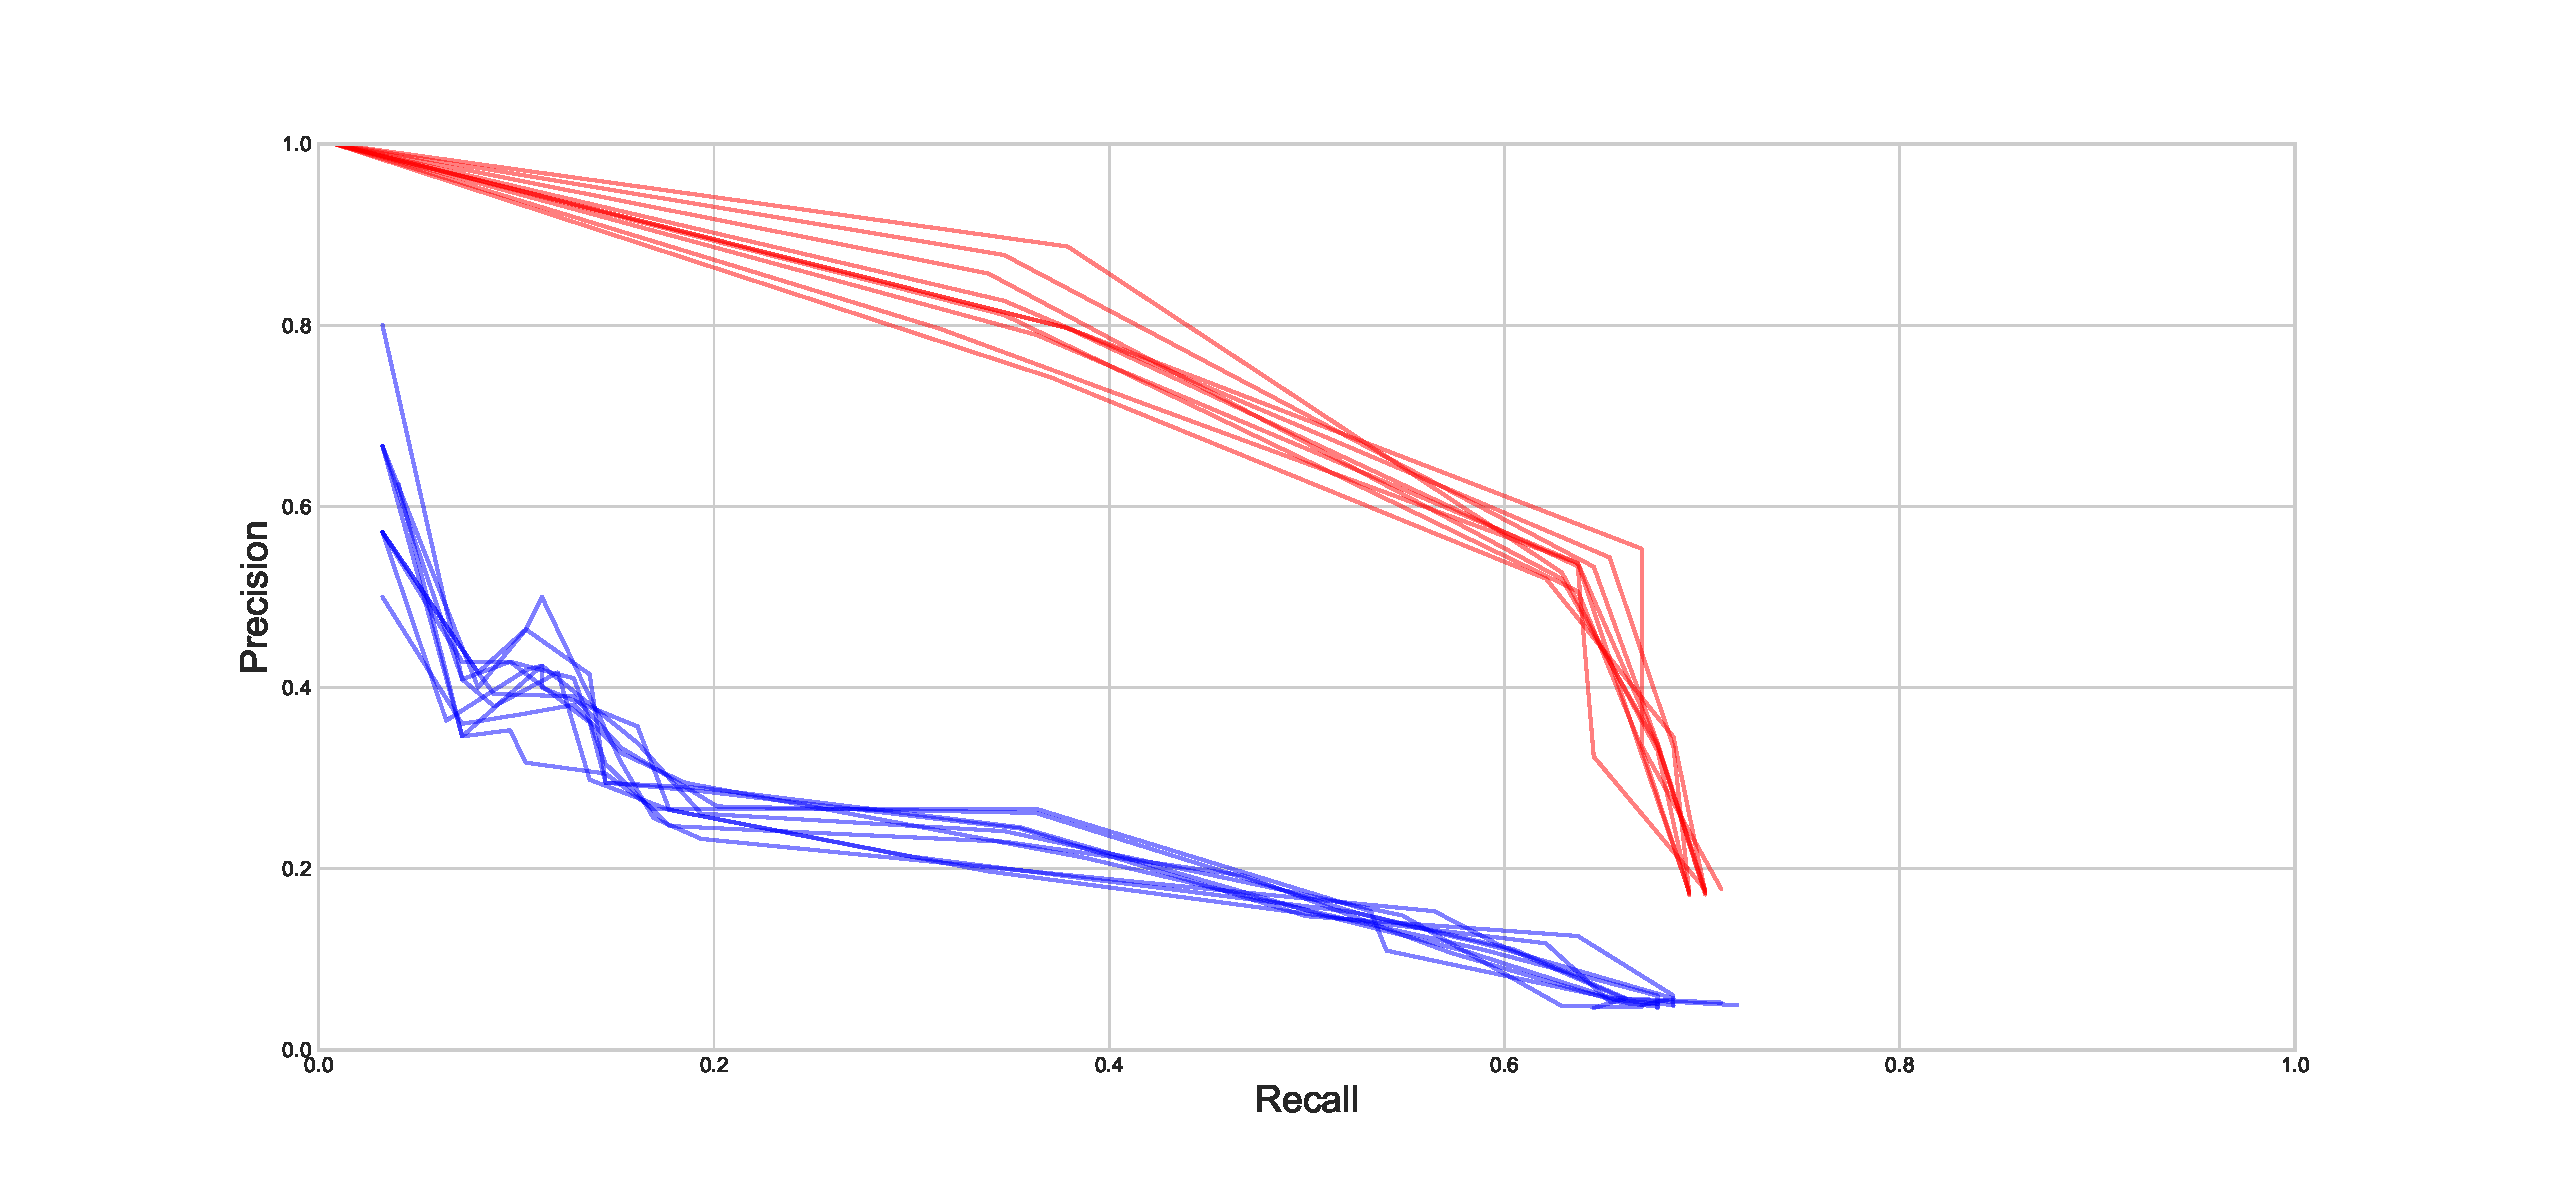
\includegraphics[width=.5\linewidth]{images/3.pdf}
		%\end{subfigure}
		\label{fig:perf}
		\end{figure}

		We then use our technique on real Ovarian Cancer data,
		and find that the support chosen by GSLR is qualitatively superior.

	\end{block}

	\vspace{1.0cm}

	% %%%%%%%%%%%%%%%%%%%%%%%%%%%%%%%%%%%%%%%%%%%%%%%%%%%%%%%%%%%%%%%%%%%%%%%%%%%
	\begin{block}{Conclusion}

		Source code and experimental code at \href{https://github.com/fraenkel-lab/gslr}{https://github.com/fraenkel-lab/gslr}

		\vspace{1.0cm}

		\textbf{Future Work:} Benchmark against related approaches which incorporate the feature graph.

	\end{block}

\end{column}
\end{columns}
\end{frame}
\end{document}
